\documentclass[a4paper,12pt]{book}
\usepackage{graphicx}
\usepackage{float}
\usepackage[T1]{fontenc}
\usepackage{hyperref}
\usepackage{adjustbox}
\graphicspath{ {./images/} }
\pagenumbering{gobble}

\hypersetup{
	colorlinks,
	linkcolor=red,
	urlcolor=blue}
	
\begin{document}

\author{Miłosz Wojciechowski}
\title{GoPro MAX video parser manual}
\date{\today}


\maketitle
\pagebreak
\pagenumbering{arabic}
\renewcommand{\labelenumii}{\arabic{enumi}.\arabic{enumii}}
\tableofcontents
\chapter{Introduction}
GoPro MAX video parser manual basic functionality is to extract equirectangular frames (every N frames or every N seconds) from a GoPro MAX spherical video and to do so the only things required are this program and an equirectangular video file. Download GoPro MAX video parser (exe file from \href{https://github.com/miloszwojciechowski/Warsaw-model/releases}{here}.)\\

\section{Input/Output}

\underline{Basic input is:} video file, directory to save frames, interval defining step between saved frames (in seconds or in frames).\\

\underline{Basic output:} folder with extracted frames.\\

Basic functionality may be expanded by using GoPro Telemetry extractor program which, if used, results in a total of:
\begin{itemize}
	\item Frames extraction
	\item Telemetry extraction
	\item Data visualization on a map
\end{itemize}

\underline{Extended input is:} basic input + GoPro Telemetry extractor program location and .LRV version of a video you are extracting frames from. LRV video has to be located in the same directory as the video you've chosen using "Choose video file" button. If you don't know what .LRV video is go to \hyperref[sec:video]{GoPro video types section}\\

\underline{Extended output is:} basic output + a csv file containing telemetry data (date, timestamp, latitude, longitude and altitude) + csv file with frames attached to their coordinates (it resembles telemetry csv, but has 2 additional columns: cts and images, former is a timestamp column calculated by the program using GoPro time register and the latter contains extracted frames paths) and visualization on a map using map html file.

\section{File structure}
\begin{itemize}
	\item Telemetry file:
	\begin{enumerate}
		\item Date: year-month-day T hour:minute:second.millisecond Z
		\item Timestamp: in milliseconds
		\item Latitude: in degrees in WGS84
		\item Longitude: in degrees in WGS84
		\item Altitude: in meters
	\end{enumerate}
	
	\item GPS file:
	\begin{enumerate}
		\item Column without a name, index column created during video processing
		\item Date: year-month-day T hour:minute:second.millisecond Z
		\item Timestamp: in milliseconds
		\item Latitude: in degrees in WGS84
		\item Longitude: in degrees in WGS84
		\item Altitude: in meters
		\item Cts: timestamp calculated from Date column, in milliseconds
		\item Images: paths to frames located in a computer memory
	\end{enumerate}
\end{itemize}

\pagebreak
List of requirements:
\begin{itemize}
	\item GoPro MAX camera
	\item Computer with at least a Windows 10 operating system
\end{itemize}
And for full functionality following additions are required:
\begin{itemize}
	\item Telemetry extractor
\end{itemize}
To get full functionality of this program and receive map visualization follow instructions from \href{https://github.com/miloszwojciechowski/Open-vslam-project/tree/main/Manuals/Telemetry_extractor}{Telemetry Extractor manual} before proceeding further. If you've followed Telemetry Extractor manual, you can skip chapters 2 and 3 (Update GoPro MAX camera, Recording a video).
\chapter{Update GoPro MAX camera}
First of all you need to update your GoPro MAX before recording anything, following steps will show how to do this:
\begin{enumerate}
	\item Download and install the GoPro app on your mobile device (from \href{https://apps.apple.com/us/app/gopro-app/id561350520}{Apple App Store} on iOS or \href{https://play.google.com/store/apps/details?id=com.gopro.smarty&hl=en}{Google Play Store} on Android)
	\item Ensure that your camera is fully charged or with at least \verb|80%| remaining power
	\item Pair your camera with the GoPro app:
	\begin{itemize}
		\item Open GoPro app on your mobile device
		\item \begin{minipage}[t]{\linewidth}
			\raggedright
			\adjustbox{valign=t}{%
				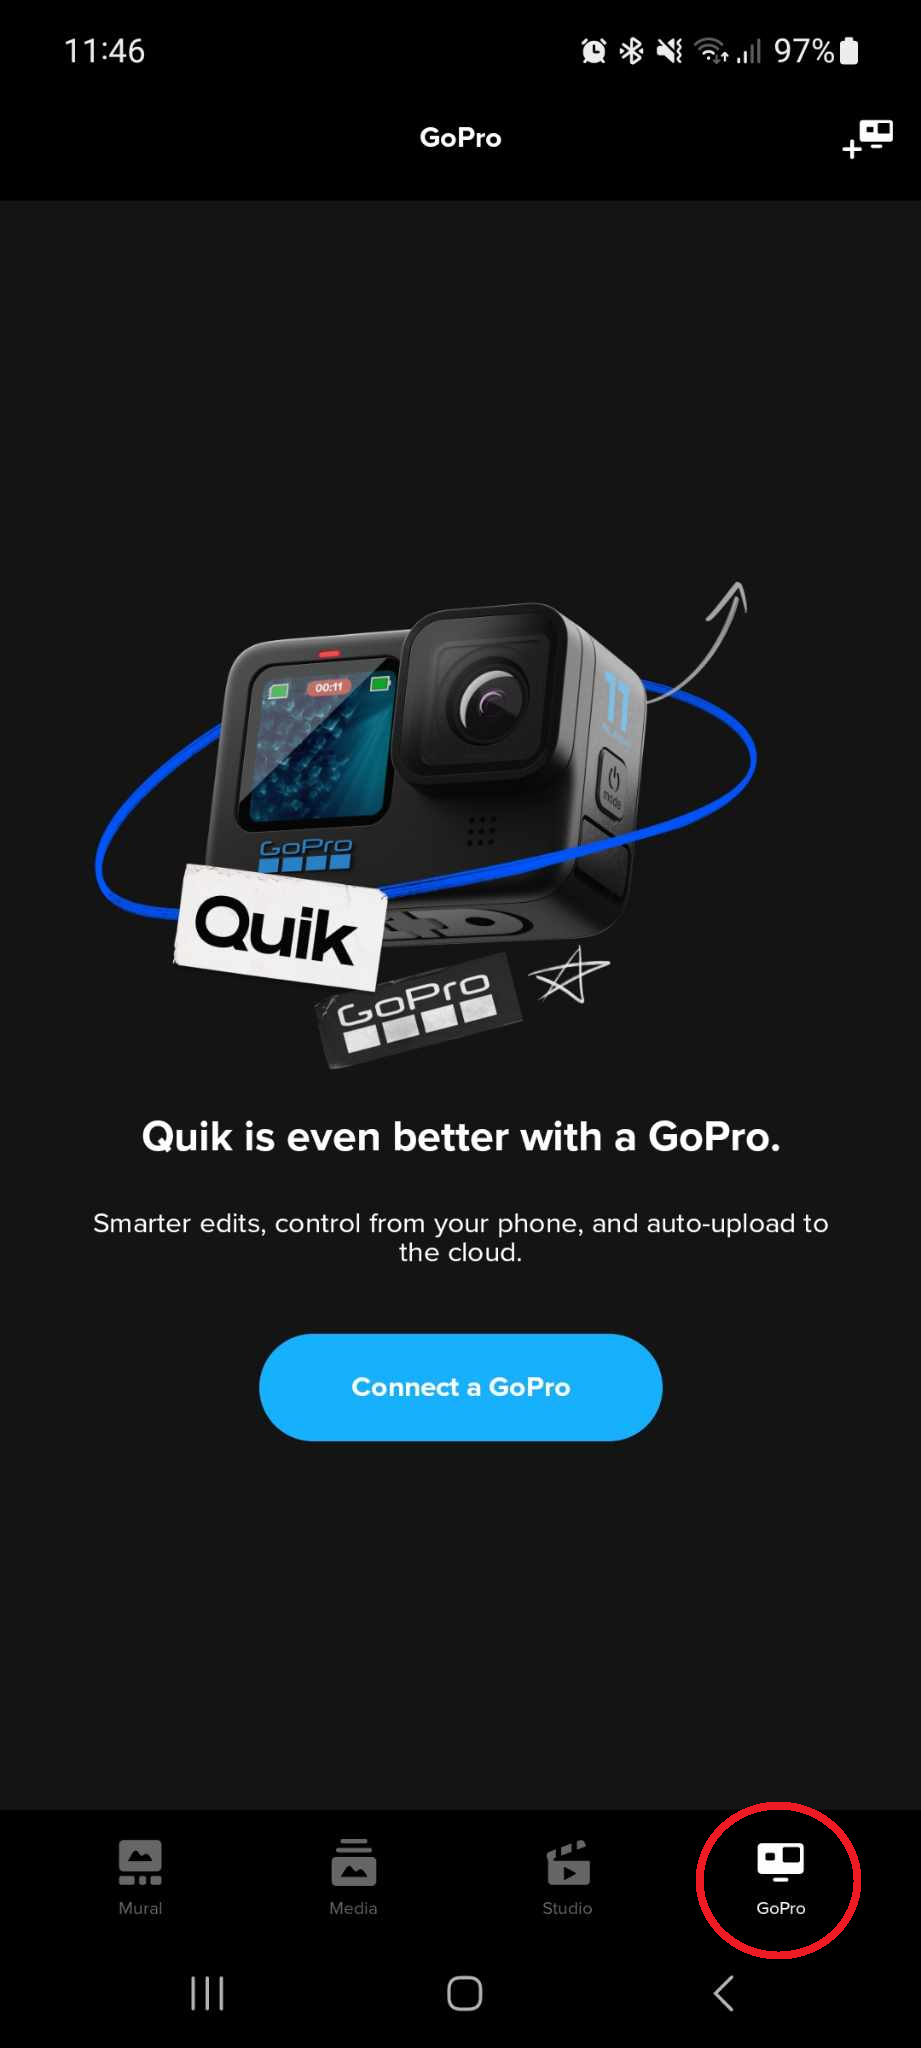
\includegraphics[width=.8\linewidth]{gopro_update1}%
			}		
			\medskip	
		\end{minipage}
		Go to GoPro tab and click Connect a GoPro, choose MAX camera and follow the instructions
		\item If an update is available, the GoPro app will prompt you to update your camera
	\end{itemize}
\end{enumerate}

\chapter{Recording a video}
\section{How to record a video}
\begin{enumerate}
	\item Record a video with your GoPro camera using the following modes:
	\begin{itemize}
		\item Traditional video in HERO or 360 mode
		\item Time Lapse in HERO or 360 mode
	\end{itemize}
	How to use GoPro MAX camera is described in the GoPro MAX manual (link in the introduction). Make sure that you have turned on GPS function otherwise video won't have telemetry data:
	\begin{figure}[H]
		\centering
		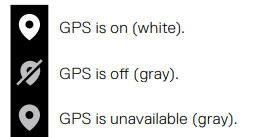
\includegraphics{GoPro_manual_fragment}
		\caption{GoPro Max manual fragment.}
	\end{figure}
	If GPS is off, swipe down to access the Dashboard and Preferences. Click on the Preferences, find option Regional and there turn the GPS On.\\
\end{enumerate}

\section{GoPro video types}
\label{sec:video}
File structure of GoPro Max videos:\\	
GoPro Max creates different types of files during recording, in 360 mode we get:
\begin{itemize}
	\item .360 file (main video file)
	\item .THM file (thumbnail file)
	\item .LRV file (low-res video file)\\
\end{itemize}
In HERO mode (traditional video in 1080p or 1440p) we get:
\begin{itemize}
	\item .MP4 file (main video file)
	\item .THM file (thumbnail file)
	\item .LRV file (low-res video file)\\
\end{itemize}
These files always appear after recording a classical video or a Time Lapse.\\

\section{Export camera recordings}
\begin{enumerate}
	\item Turn on your GoPro camera.
	\item Open your GoPro MAX side panel and connect it to your computer using USB 2.0 to USB-c cable included in a camera set. Information as below should display on the screen:
	\begin{figure}[H]
		\centering
		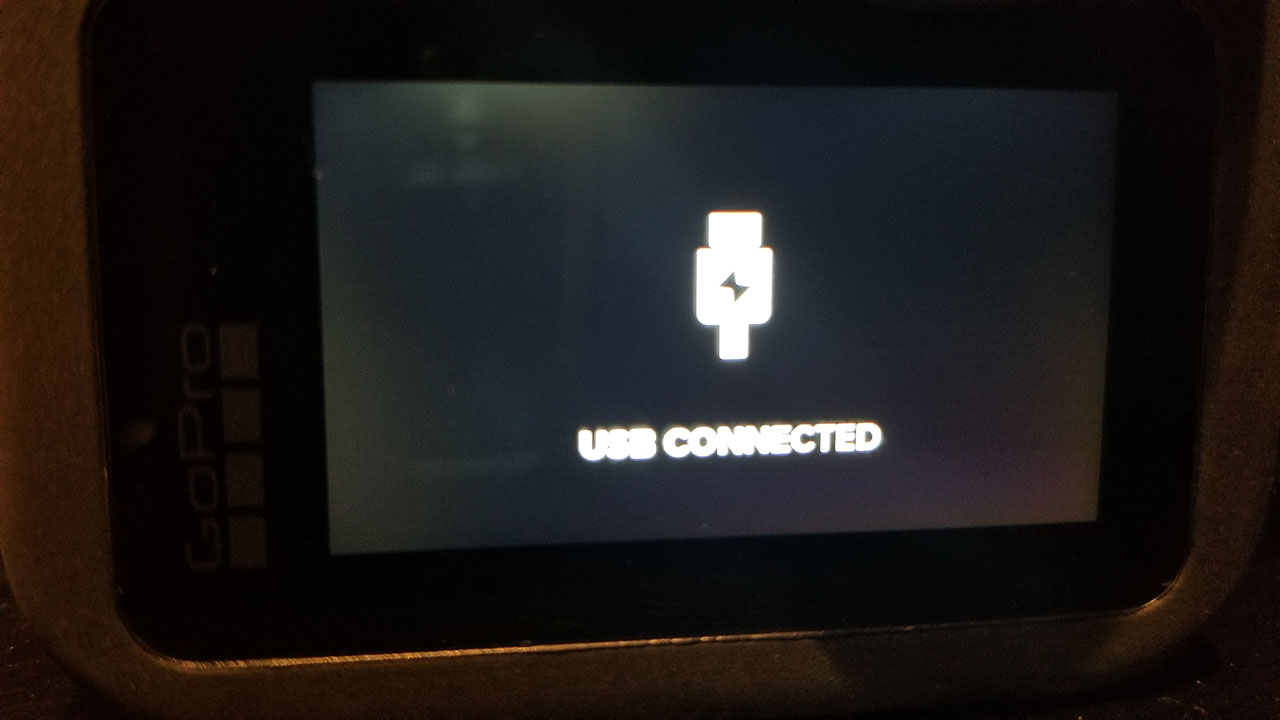
\includegraphics{camera_connected}
		\caption{Successfully connected camera.}
	\end{figure} 
	
	\item Now find your connected GoPro camera and navigate through directories:\\
	
	$\textit{GoPro MAX > GoPro MTP Client Disk Volume > DCIM > 100GOPRO}$	\\
	
	Final path should look like this:
	
	\textit{GoPro MAX/GoPro MTP Client Disk Volume/DCIM/100GOPRO}	
	\begin{figure}[H]
		\centering
		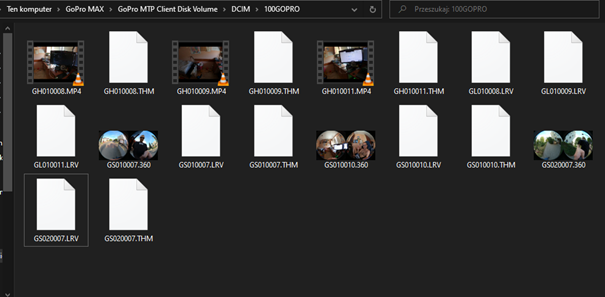
\includegraphics{recording_location}
		\caption{Video files location.}
	\end{figure}
	\hfill
	\item 360 videos’ names and their LRV versions start with GS e.g. GS020007.360, GS020007.LRV.\\
	
	Regular videos’ and their LRV versions’ names start with GH for the former and with GL for the latter e.g. GH010008.MP4, GL010008.LRV. \\
	\item Copy videos of your choice and save them on your computer.
\end{enumerate}

\chapter{Install FFmpeg}
\begin{enumerate}
	\item Go to \url{https://ffmpeg.org/download.html}
	\item \begin{minipage}[t]{\linewidth}
		\raggedright
		\adjustbox{valign=t}{%
			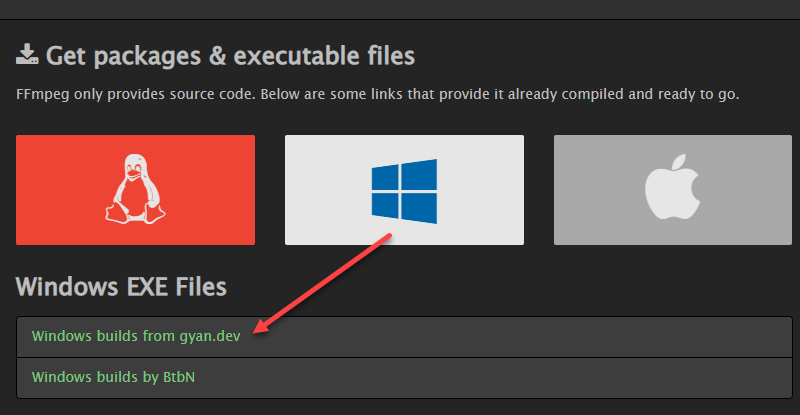
\includegraphics[width=.8\linewidth]{ffmpeg_install1}%
		}		
		\medskip	
	\end{minipage}
	To download Windows version click on the windows symbol and then choose Windows builds from gyan.dev
	\item \begin{minipage}[t]{\linewidth}
		\raggedright
		\adjustbox{valign=t}{%
			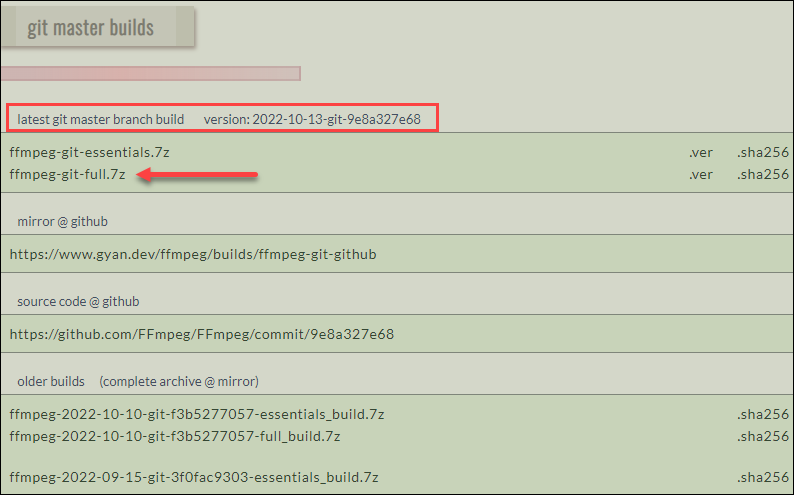
\includegraphics[width=.8\linewidth]{ffmpeg_install2}%
		}		
		\medskip	
	\end{minipage}
	On the new site choose latest git master branch build and download full version of ffmpeg
	\item Unpack the downloaded zip file in a directory of your choice
	\item Add FFmpeg to PATH:
	\begin{itemize}
		\item Press Windows+R and type "sysdm.cpl", window will pop up, go to "Advanced" tab and there press "Environment variables".
		\item \begin{minipage}[t]{\linewidth}
			\raggedright
			\adjustbox{valign=t}{%
				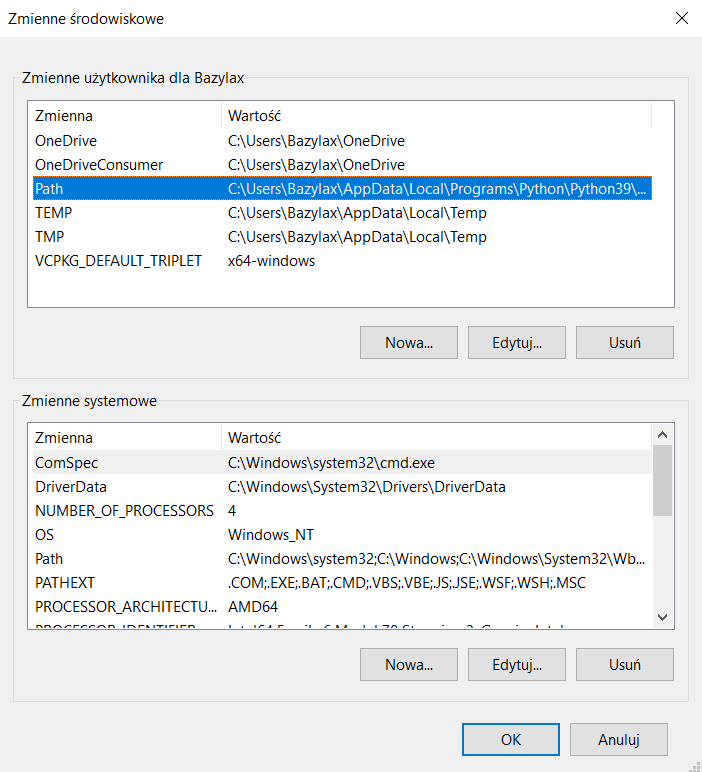
\includegraphics[width=.8\linewidth]{python_install6}%
			}		
			\medskip	
		\end{minipage}
		Window as above should pop up, click on the Path.
		\item \begin{minipage}[t]{\linewidth}
			\raggedright
			\adjustbox{valign=t}{%
				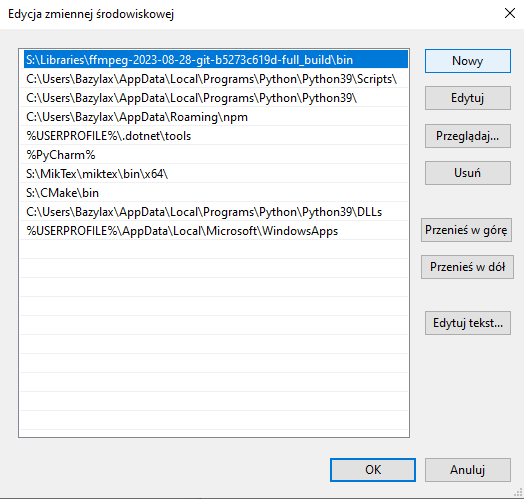
\includegraphics[width=.8\linewidth]{ffmpeg_install3}%
			}		
			\medskip	
		\end{minipage}
		Click New and paste path to \verb|\ffmpeg\bin| which contains ffmpeg.exe. Then confirm changes by pressing ok. After adding ffmpeg to PATH restart your computer.
		\item To check if installed correctly open Command Prompt (by writing cmd in the start menu) and write "ffmpeg"
	\end{itemize}
\end{enumerate}

\chapter{Prepare equirectangular video}
\begin{enumerate}
	\item Download and install Go Pro Player app \url{https://gopro.com/en/us/info/gopro-player}
	\item If you don't have HEVC video extension, use the installer located in \verb|HEVC_video_extension| provided within the main repository.
	\item Open .360 video in the GoPro Player
	 \item \begin{minipage}[t]{\linewidth}
	 	\raggedright
	 	\adjustbox{valign=t}{%
	 		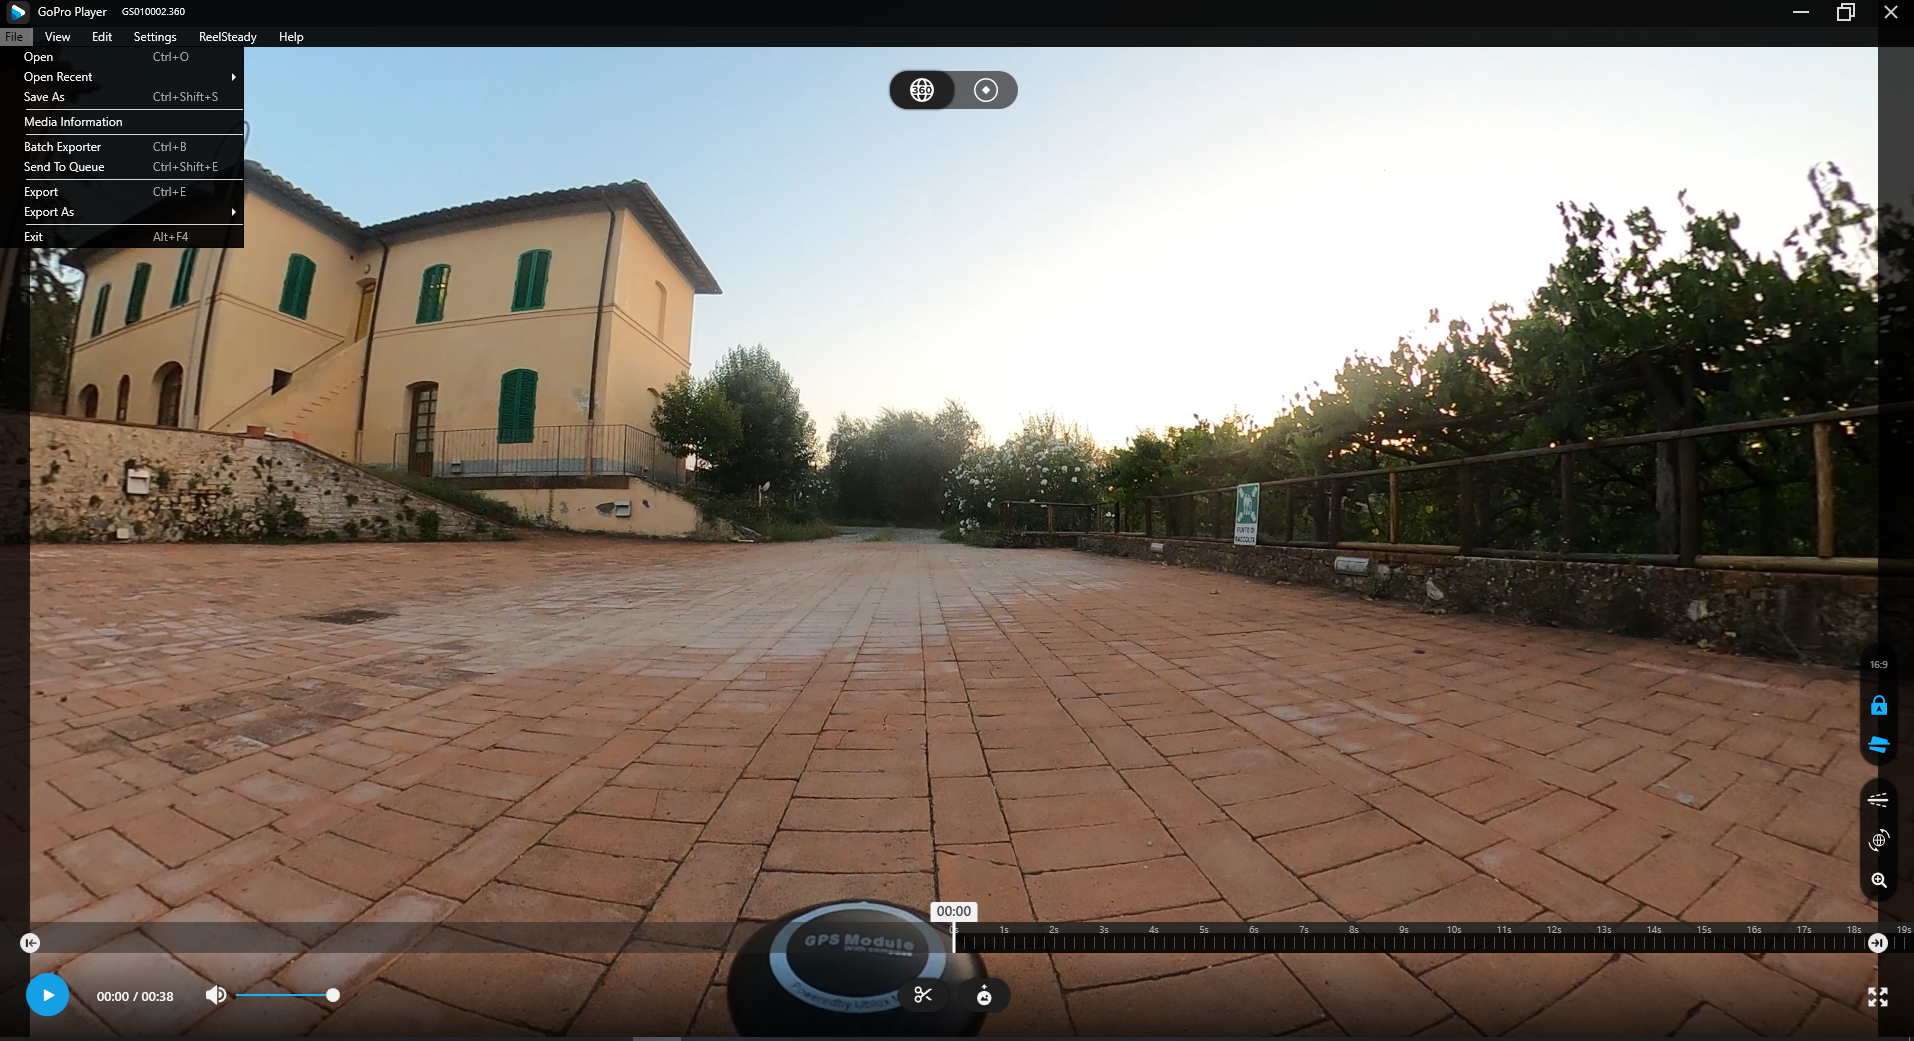
\includegraphics[width=.8\linewidth]{player1}%
	 	}		
	 	\medskip	
	 \end{minipage}
	 Go to File
	 \item \begin{minipage}[t]{\linewidth}
	 	\raggedright
	 	\adjustbox{valign=t}{%
	 		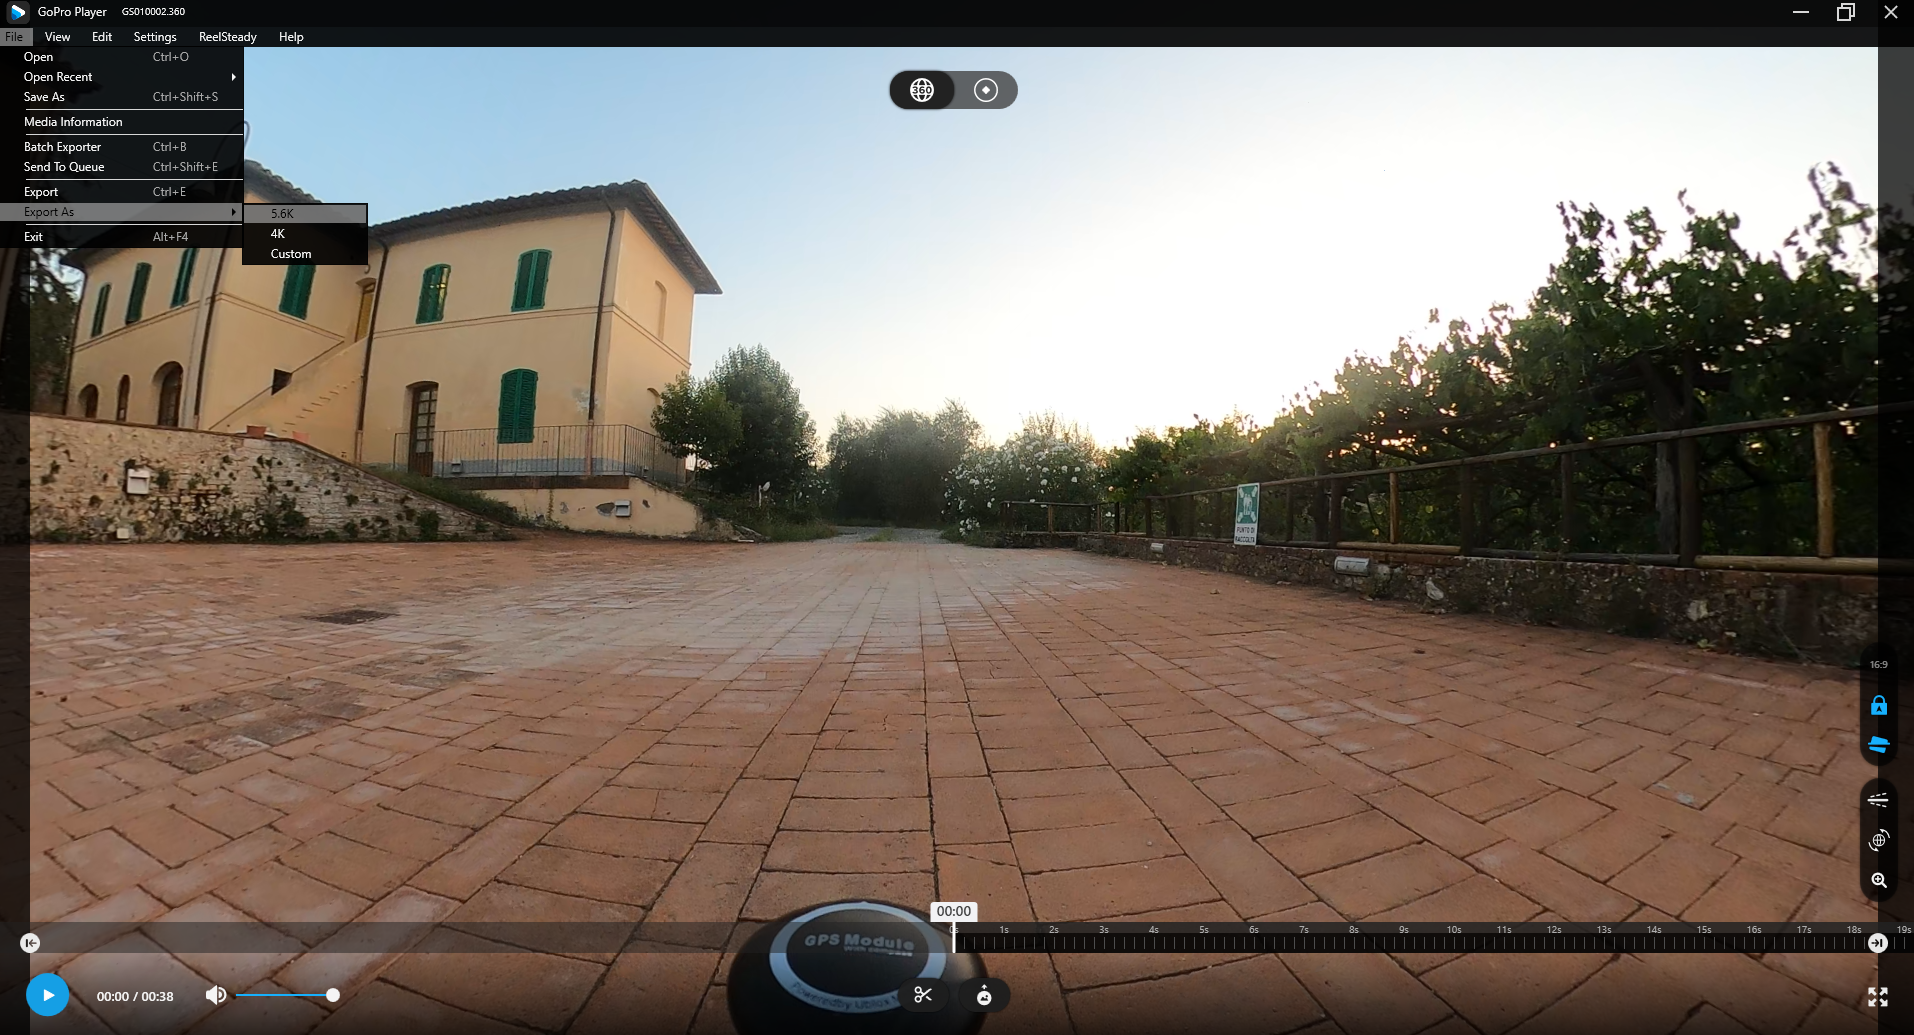
\includegraphics[width=.8\linewidth]{player2}%
	 	}		
	 	\medskip	
	 \end{minipage}
	 Choose Export as > 5.6K
	 \item \begin{minipage}[t]{\linewidth}
	 	\raggedright
	 	\adjustbox{valign=t}{%
	 		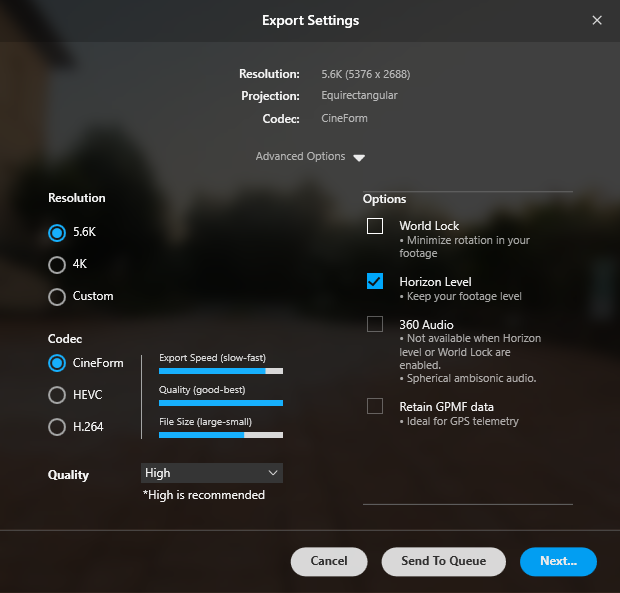
\includegraphics[width=.8\linewidth]{player3}%
	 	}		
	 	\medskip	
	 \end{minipage}
	 Disable World Lock, make sure 5.6K and CineForm are chosen. Click Next, choose directory where equirectangular video will be created and wait for the Player to do the job.
\end{enumerate}
\chapter{Run the program}
\begin{enumerate}
	\item \begin{minipage}[t]{\linewidth}
		\raggedright
		\adjustbox{valign=t}{%
			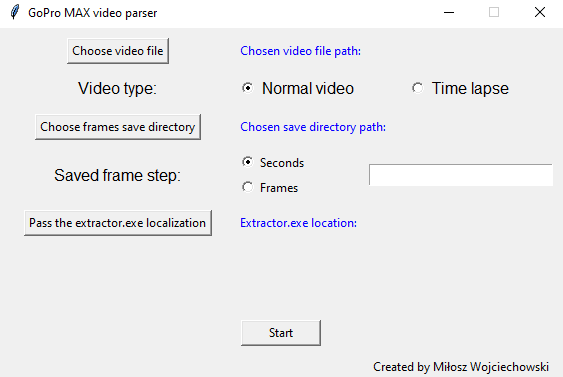
\includegraphics[width=.8\linewidth]{window1}%
		}		
		\medskip	
	\end{minipage}
	After running GoPro\_MAX\_video\_parser.exe application window should open.
	There can be seen a few buttons and an input area:
	\begin{itemize}
		\item \textbf{Choose video file} - open file explorer and select video file. As opposed to telemetry extractor it is recommended to avoid .LRV file since extracted frames should be the highest possible quality.
		\item \textbf{Video type} - choose whether you parse normal video or time lapse (for the difference check \url{https://gopro.com/content/dam/help/max/manuals/MAX_UM_ENG_REVB.pdf}). If time lapse is chosen, pass the interval (in seconds) you chose on your GoPro camera (default is 0.5s), additionaly the saved frame step choice is locked and the only possible one is Frames.
		\item \textbf{Choose Frames save director}y - open file explorer and choose directory which extracted frames will be saved to. Make sure chosen folder is empty or create a new empty one.
		\item \textbf{Saved frame step} - first decide whether passed value should be number of seconds between extracted frames or number of frames between extracting extracted frames  e.g. when set to Seconds and number 30 is passed the program will extract one frame every 30 seconds but when set to Frames the program will extract one frame every 30 frames, so for video recorded in 30 FPS program will extract a frame every one second.
		\item \textbf{Pass the extractor.exe localization} - to use only when Telemetry extractor was installed. Open file explorer and choose extractor.exe localization (when using program with this function remember to put both .mov and .LRV files in the same folder), if not passed,  warning will pop up asking whether to run the application without extractor.exe. If answered yes, only frames will be extracted.
		\item \textbf{Start} - run the program, before that make sure you filled all the needed data (video file, save directory and frame step). If running with extractor.js make sure that .LRV file is in the same directory as video file you provided via "Choose video file" button.
	\end{itemize}
	\item \begin{minipage}[t]{\linewidth}
		\raggedright
		\adjustbox{valign=t}{%
			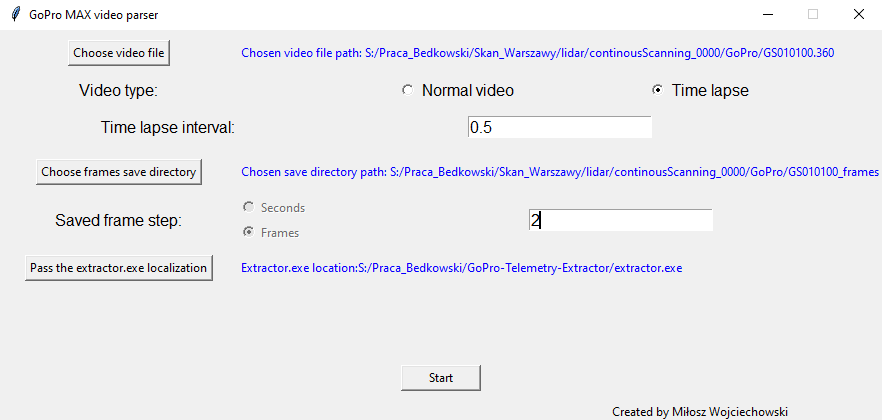
\includegraphics[width=.8\linewidth]{window2}%
		}		
		\medskip	
	\end{minipage}
	After filling all the needed data press "Run" button. A console will open showing frames extraction process. If you want to stop it, press "Q". If extractor.js was provided, a csv file with telemetry data will appear in the directory of the provided video along with a csv frames file. Additionally a map will open, which has the source file in the folder Maps created in video parser directory after the first usage.\\
	If you run into \textbf{Couldn't extract telemetry data} error it might be caused by one of the below:
	\begin{itemize}
		\item No .LRV file in the folder
		\item Telemetry csv file is not closed
	\end{itemize}
\end{enumerate}
\end{document}